\subsection{Experiment Interfaces}

\subsubsection{Mechanical Interfaces}
The experiment box will be fixed to the gondola rails by means of 4 screws interfacing the experiment outside structure with the hammer nuts in the rails. 90-degree aluminum angles will be used to provide this interface.This method is secure as well as fast enough to provide an accessible and easy recuperation for the later analysis. 

Lateral and top handles will be mounted to facilitate the experiment box manipulation when moving it in and out of the gondola. 

In order to collect reliable air samples, the experiment requires to be mounted at least with one side exposed to the outside. The later will reduce the pipe length used to collect clean air. Three tubes will extend from the experiment box face, see Figures \ref{fig:pipes_interface} and \ref{fig:pipes_interface_1}. One for the CAC sampling and two, input and output, for the AAC sampling. The one-way selected method will provide a proper flushing of the pipe and thus ensure a reliable sampling as explained in section \ref{Experiment_Setup}.

\bigskip

\subsubsection{Electrical Interfaces}
\begin{centering}
The experiment will connect to the gondola electrically via a 4 pin, male, box mount receptacle MIL - C-26482P series 1 connector with an 8-4 insert arrangement (MS3112E8-4P) \cite{BexusManual}. It will connect to one 28.8V/1mA battery pack which consists of eight SAFT LSH20 batteries in series where each has a 5A fuse\cite{BexusManual}. The expected maximum current is 1.33A.
\end{centering}
\bigskip

\begin{centering}
The E-Link connection shall be made between the experiment and the E-Link system using a RJ45 connection which will be supplied by SSC and an Ethernet protocol. The Amphenol RJF21B connector will be mounted on either the front or the side of the experiment\cite{BexusManual}.  
\end{centering}
\bigskip

\begin{centering}
The expected data rate is 2kbit/s with 10kbit/s peak downlink and 5kbit/s peak uplink.
\end{centering}

\begin{figure}[H]
    \begin{align*}
        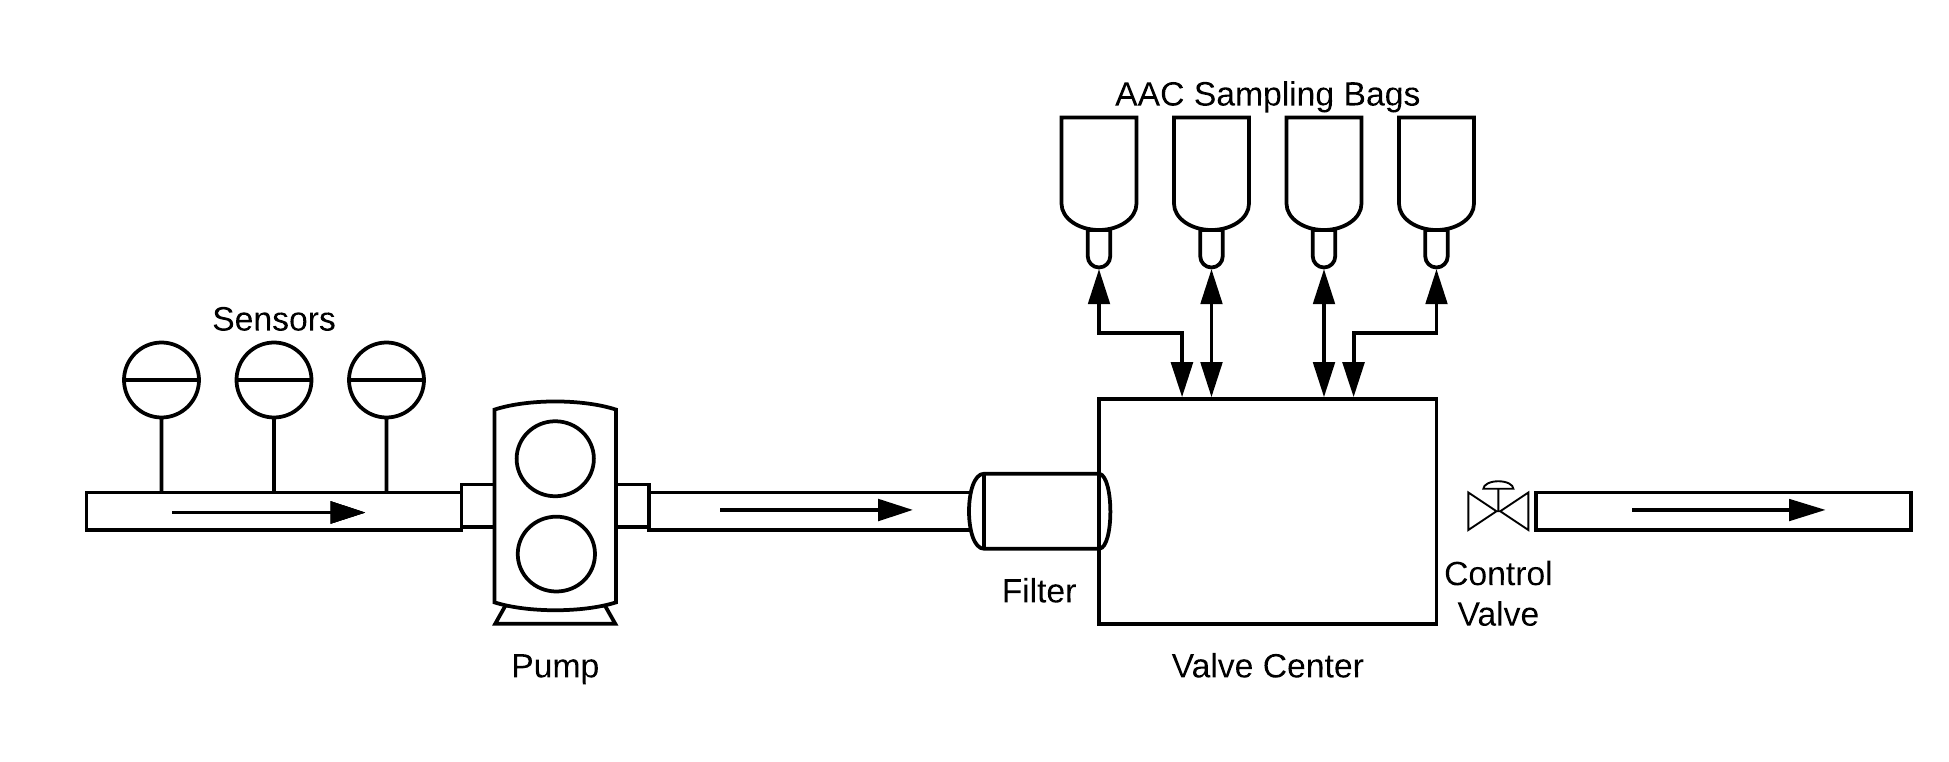
\includegraphics[width=0.7\textwidth]{4-experiment-design/img/Schematic_pipe.png}
    \end{align*}
    \caption{Schematic of air sampler pipe.}\label{fig:pipes_interface}
\end{figure}

\begin{figure}[H]
    \begin{align*}
        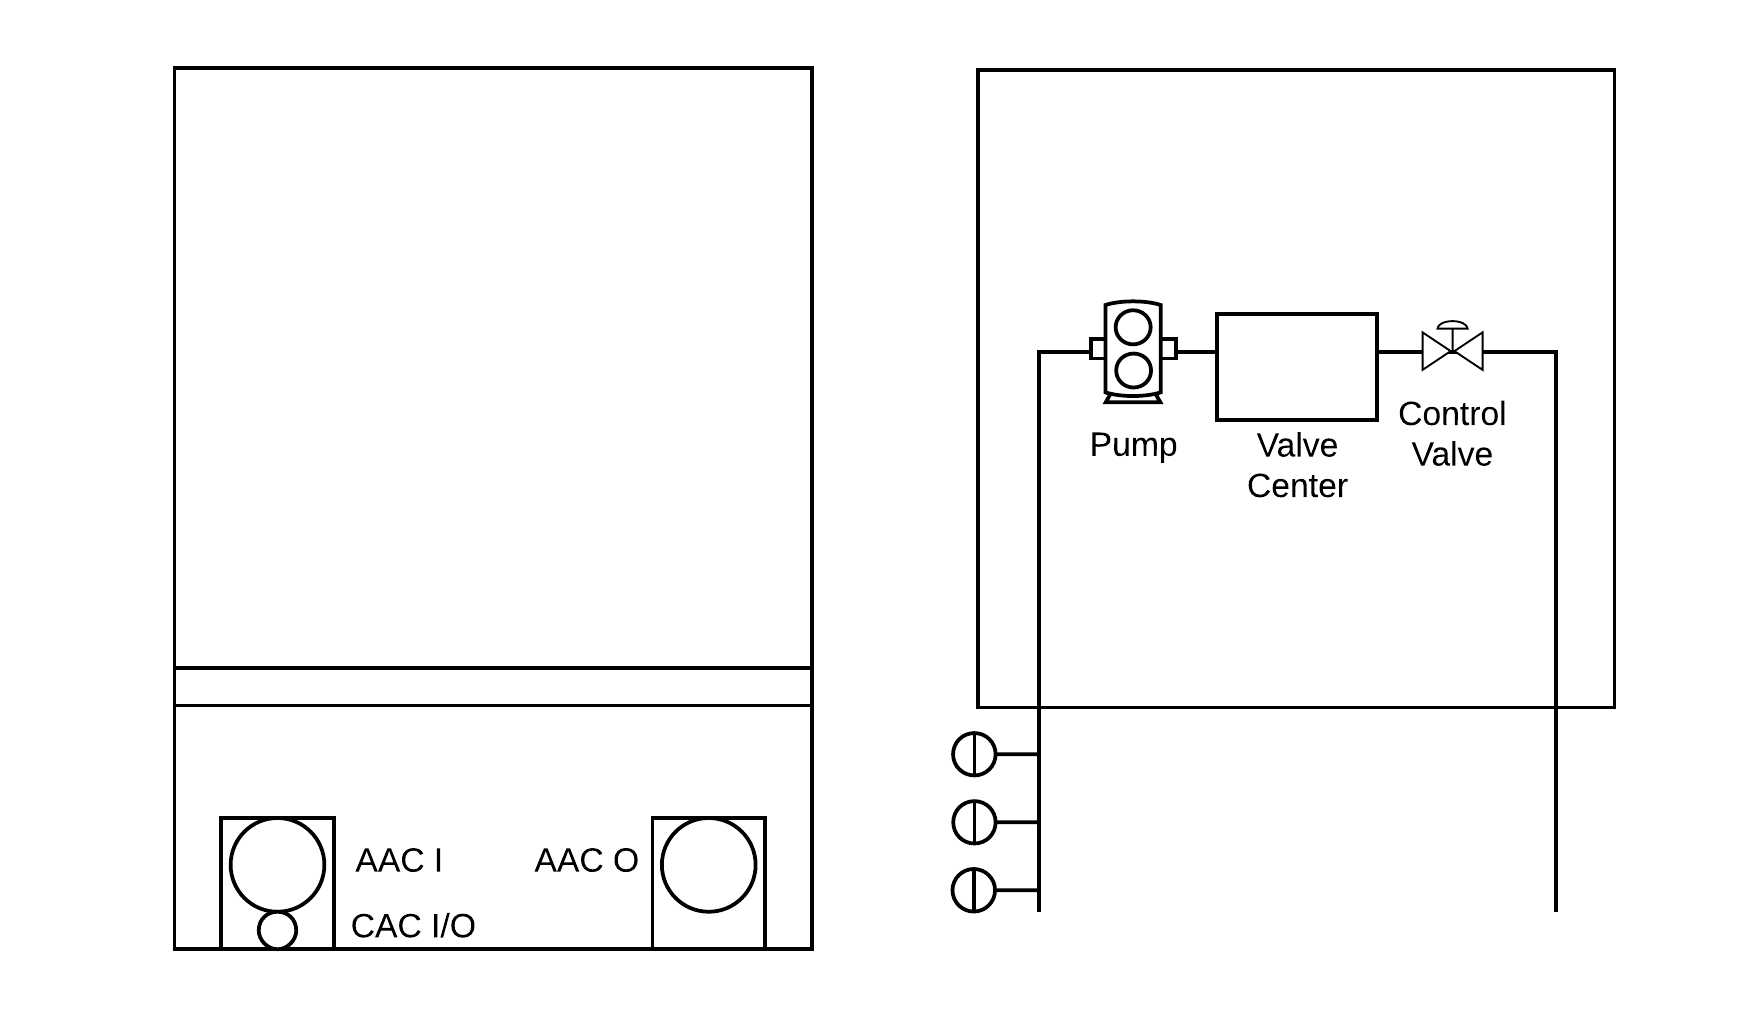
\includegraphics[width=0.7\textwidth]{4-experiment-design/img/Diagram_pipe.png}
    \end{align*}
    \caption{Diagram of the experiment box face exposed to the outside.}\label{fig:pipes_interface_1}
\end{figure}

\iffalse
\subsubsection{Radio Frequencies (Optional)}
\begin{centering}
Not required.
\end{centering}
\bigskip

\subsubsection{Thermal (Optional)}
\begin{centering}
Not required.
\end{centering}
\bigskip
\fi


\raggedbottom